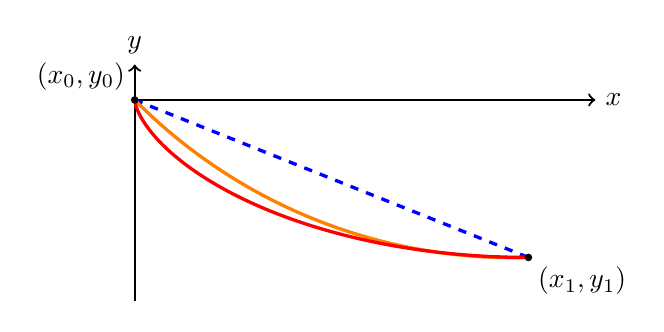
\begin{tikzpicture}[scale=1.0]
  % y upward; three curves share the endpoints
  \draw[->, thick] (0,0) -- (5.85,0) node[right] {$x$};
  \draw[->, thick] (0,-2.55) -- (0,0.45) node[above] {$y$};

  \coordinate (A) at (0,0);
  \coordinate (B) at (5,-2);

  % straight chord
  \draw[blue, dashed, very thick] (A) -- (B);
  % circular arc through A and B, bulging below the chord
  \draw[orange, very thick, domain=-135.28:-88.33, samples=80, smooth]
    plot ({4.8026+6.7594*cos(\x)}, {4.7566+6.7594*sin(\x)});
  % steep curve: cycloid half-arch stretched to the same endpoints
  \draw[red, very thick, domain=0:3.1416, samples=100, smooth]
    plot ({(5/3.1416)*(\x - sin(\x r))}, {cos(\x r) - 1});

  \filldraw (A) circle (1.15pt) node[above left] {$(x_0,y_0)$};
  \filldraw (B) circle (1.15pt) node[below right] {$(x_1,y_1)$};
\end{tikzpicture}
